\documentclass[12pt]{article}
\usepackage[margin=1in]{geometry} 
\usepackage{amsmath,amsthm,amssymb,amsfonts,mathtools,tikz,gensymb}
\usepackage[makeroom]{cancel}
\graphicspath{ {./figures/} }

\newenvironment{problem}[2][]{
    \begin{trivlist}
        \item[
            {\bfseries #1}
            {\bfseries #2.}
        ]
}{\end{trivlist}}

\pagenumbering{gobble}

% --------------------------------------------------
% CUSTOM COMMANDS
% -------------------------------------------------- 

\newcommand{\assignment}{Pg. 595 \#3-24, 25, 27, 29, 31, 32}
\newcommand{\name}{Eric Nguyen}
\newcommand{\duedate}{2019-05-09}
\newcommand{\details}{\noindent\textbf{\name \\\duedate \\\assignment}}

\newcommand{\Problem}[1]{\bigskip \noindent #1}
\newcommand{\Part}[1]{\shortintertext{(#1)}}
\newcommand{\dx}{\, dx}
\newcommand{\dy}{\, dy}
\newcommand{\dv}{\, dv}
\newcommand{\dt}{\, dt}
\newcommand{\descprob}[1]{\hfill\break #1}
\newcommand{\plugin}[2]{\left(\left({#1}\right) - \left({#2}\right)\right)}
\newcommand{\setuv}[4]{
\left[
\begin{alignedat}{2}
u &= #1 &\quad v &= #3 \\
du &= #2 &\quad dv &= #4 \\
\end{alignedat}
\right]  = uv - \int v ~ du \\
&= \intbp{#1}{#3}{#2}
}
\newcommand{\subu}[2]{
\left[
\begin{alignedat}{1}
u &= #1 \\
du &= #2 \\
\end{alignedat}
\right] 
}
\newcommand{\intbp}[3]{\left(#1\right) \left(#2\right) - \int \left(#2\right) \left(#3\right)}
\newcommand{\descmeet}{\shortintertext{\quad Find where the graphs meet:}}
\newcommand{\deschigh}{\shortintertext{\quad Find the graph that is higher between the interval:}}
\newcommand{\descarea}{\shortintertext{\quad Find the area of the difference of the two graphs between the interval:}}

% --------------------------------------------------  
% TABULAR INTEGRATION
% -------------------------------------------------- 	

\usepackage{booktabs}
\usepackage{xparse}
\usepackage{tikz}
\usetikzlibrary{calc}

\tikzset{Arrow Style/.style={text=black, font=\boldmath}}

\newcommand{\tikzmark}[1]{%
    \tikz[overlay, remember picture, baseline] \node (#1) {};%
}

\newcommand*{\XShift}{0.5em}
\newcommand*{\YShift}{0.5ex}

\NewDocumentCommand{\DrawArrow}{s O{} m m m}{
    \begin{tikzpicture}[overlay,remember picture]
        \draw[->, thick, Arrow Style, #2] 
                ($(#3.west)+(\XShift,\YShift)$) -- 
                ($(#4.east)+(-\XShift,\YShift)$)
        node [midway,above] {#5};
    \end{tikzpicture}
}

\begin{document}

\details

\begin{problem}{3}
    \textbf{a)} Graph: $f(x) = \left\{
        \begin{array}{ll}
            5 - x, & \text{for } x \neq 2, \\
            -3, & \text{for } x = 2.
        \end{array}\right.$ \\
    \indent\,\,\,\textbf{b)} Find $\underset{x \to 2}{\lim} f(x)$. \\
    \indent\,\,\,\textbf{c)} Find f(2). \\
    \indent\,\,\,\textbf{d)} Is $f$ continuous at 2? \\
    \begin{align*}
        \Part{a}
        &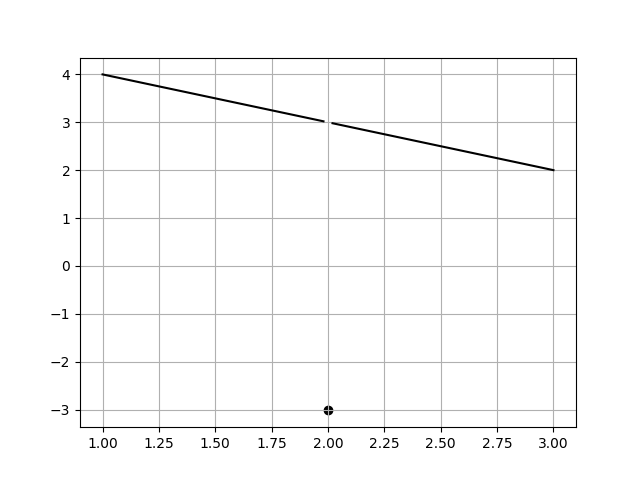
\includegraphics[scale=0.65]{595_03.png}
    \end{align*}
    \begin{align}
        \Part{b}
        \underset{x \to 2}{\lim} &= 3
        \Part{c}
        f(2) &= -3
        \Part{d}
        \text{No, } f \text{ is not } & \text{continuous at 2. }
    \end{align}
\end{problem}

\clearpage

\Problem{Find each limit, if it exists. If a limit does not exist, state that fact.}

\begin{problem}{4}
    $\underset{x \to -4}{\lim} \dfrac{x^2 - 16}{x + 4}$
    \begin{align}
        \frac{(-4.1)^2 - 16}{(-4.1) - 16} &= -8.1 \\
        \frac{(-3.9)^2 - 16}{(-3.9) - 16} &= -7.9 \\
        \underset{x \to -4}{\lim} \frac{x^2 - 16}{x + 4} &= \text{Does not exist.}
    \end{align}
\end{problem}

\begin{problem}{5}
    $\underset{x \to 1}{\lim} \sqrt{x^3 + 8}$
    \begin{align}
        \sqrt{0.9^3 + 8} &\approx 2.95 \\
        \sqrt{1.1^3 + 8} &\approx 3.05 \\
        \underset{x \to 1}{\lim} \sqrt{x^3 + 8} &= 3 
    \end{align}
\end{problem}

\begin{problem}{6}
    $\underset{x \to 3}{\lim} \, \dfrac{4}{x - 3}$
    \begin{align}
        \frac{4}{2.9 - 3} &= -40 \\
        \frac{4}{3.1 - 3} &= 40 \\
        \underset{x \to 3}{\lim} \, \frac{4}{x - 3} &= \text{Does not exist.}
    \end{align}
\end{problem}

\begin{problem}{7}
    $\underset{x \to \infty}{\lim} \dfrac{12x - 7}{3x + 2}$
    \begin{align}
        \frac{12 \left(10000\right) - 7}{3 \left(10000\right) + 2} &\approx 4 \\
        \underset{x \to \infty}{\lim} \dfrac{12x - 7}{3x + 2} &= 4
    \end{align}
\end{problem}

\begin{problem}{8}
    $\underset{x \to \infty}{\lim} \, \dfrac{2x^3 - x}{8x^5 - x^2 + 1}$
    \begin{align}
        \frac{2\left(10000\right)^3 - \left(10000\right)}{8\left(10000\right)^5 - \left(10000\right)^2 + 1} &\approx 0 \\
        \underset{x \to \infty}{\lim} \, \frac{2x^3 - x}{8x^5 - x^2 + 1} &= 0
    \end{align}
\end{problem}

\begin{problem}{9}
    If $f(x) = x^2 + 3$, find $f'(x)$ by determining $\underset{h \to 0}{\lim} \dfrac{f(x + h) - f(x)}{h}.$
    \begin{align}
        &= \underset{h \to 0}{\lim} \frac{\left(x + h\right)^2 + 3 - x^2 - 3}{h} \\
        &= \underset{h \to 0}{\lim} \frac{x^2 + 2xh + h^2 - x^2}{h} \\
        &= \underset{h \to 0}{\lim} \, 2x + h \\
        &= 2x
    \end{align}
\end{problem}

\Problem{Differentiate.}

\begin{problem}{10}
    $y = -9x + 3$
    \begin{align}
        &= -9
    \end{align}
\end{problem}

\begin{problem}{11}
    $y = x^2 - 7x + 3$
    \begin{align}
        &= 2x - 7
    \end{align}
\end{problem}

\begin{problem}{12}
    $y = x^{1/4}$
    \begin{align}
        &= \frac{1}{4} x^{-3/4}
    \end{align}
\end{problem}

\begin{problem}{13}
    $f(x) = x^{-6}$
    \begin{align}
        &= -6x^{-7}
    \end{align}
\end{problem}

\begin{problem}{14}
    $f(x) = \sqrt[3]{2x^5 - 8}$
    \begin{align}
        &= \frac{1}{3} \left(2x^5 - 8\right)^{-2/3} \cdot 10x^4 \\
        &= \frac{10}{3} x^4 \left(2x^5 - 8\right)^{-2/3}
    \end{align}
\end{problem}

\begin{problem}{15}
    $f(x) = \dfrac{5x^3 + 4}{2x - 1}$
    \begin{align}
        &= \frac{\left(2x - 1\right) \left(15x^2\right) - \left(5x^3 + 4\right) \left(2\right)}{\left(2x - 1\right)^2} \\
        &= \frac{30x^3 - 15x^2 - 10x^3 - 8}{\left(2x - 1\right)^2} \\
        &= \frac{20x^3 - 15x^2 - 8}{\left(2x - 1\right)^2}
    \end{align}
\end{problem}

\begin{problem}{16}
    $y = \ln \left(x^2 + 5\right)$
    \begin{align}
        &= \frac{2x}{x^2 + 5}
    \end{align}
\end{problem}

\begin{problem}{17}
    $y = e^{\ln x}$
    \begin{align}
        &= \frac{1}{x} \cdot e^{\ln x} \\
        &= \frac{x}{x} = 1
    \end{align}
\end{problem}

\begin{problem}{18}
    $y = e^{3x} + x^2$
    \begin{align}
        &= 3e^{3x} + 2x
    \end{align}
\end{problem}

\begin{problem}{19}
    $y = e^{\sqrt{x - 3}}$
    \begin{align}
        &= \frac{1}{2} \left(x - 3\right)^{-1/2} e^{\sqrt{x - 3}} \\
        &= \frac{e^{\sqrt{x - 3}}}{2 \sqrt{x - 3}}
    \end{align}
\end{problem}

\begin{problem}{20}
    $f(x) = \ln \left(e^x - 4\right)$
    \begin{align}
        &= \frac{e^x}{e^x - 4}
    \end{align}
\end{problem}

\begin{problem}{21}
    For $y = x^2 - \dfrac{2}{x}$, find $d^2 y / dx^2$.
    \begin{align}
        &= \frac{d}{dx} 2x + \frac{2}{x^2} \\
        &= 2 - \frac{4}{x^3}
    \end{align}
\end{problem}

\begin{problem}{22}
    \textbf{Business: average cost.}
    Doubletake Clothing finds that the cost, in dollars, of producing $x$ pairs of jeans is given by $C(x) = 320 + 9\sqrt{x}$.
    Find the rate at which the average cost is changing when 100 pairs of jeans have been produced.
    \begin{align}
        C_{\text{av}}(x) &= \frac{320 + 9\sqrt{x}}{x} \\
        &= 320x^{-1} + 9x^{-1/2} \\
        {C_{\text{av}}}'(x) &= -320x^{-2} - \frac{9}{2} x^{-3/2} \\
        {C_{\text{av}}}'(100) &= -320\left(100\right)^{-2} - \frac{9}{2} \left(100\right)^{-3/2} \\
        &\approx \$0.04/\text{pair}
    \end{align}
\end{problem}

\begin{problem}{23}
    Differentiate implicitly to find $dy/dx$ if $x^3 + x/y = 7$.
    \begin{align}
        3x^2 + \frac{y \left(1\right) - x \left(1\right) \frac{dy}{dx}}{y^2} &= 0 \\
        3x^2y^2 + y - x \frac{dy}{dx} &= 0 \\
        3x^2y^2 + y &= x \frac{dy}{dx} \\
        \frac{dy}{dx} &= 3xy^2 + \frac{y}{x}
    \end{align}
\end{problem}

\begin{problem}{24}
    Find an equation of the tangent line to the graph of $y = e^x - x^2 - 3$ at the point (0, -2).
    \begin{align}
        y' &= e^x - 2x \\
        y_\tan &= y'(0) (x - 0) + y(0) \\
        &= \left(e^0 - 2(0)\right) \left(x - 0\right) + \left(e^0 - 0^2 - 3\right) \\
        &= x - 2
    \end{align}
\end{problem}

\Problem{Sketch the graph of each function.
List and label the coordinates of any extrema and points of inflection.
State where the function is increasing or decreasing, where it is concave up or concave down, and where any asymptotes occur.}

\begin{problem}{25}
    $f(x) = x^3 - 3x + 1$
    \begin{align}
        f'(x) &= 3x^2 - 3 \\
        f''(x) &= 6x 
        \shortintertext{Critical points}
        0 &= 3x^2 - 3 \\
        x &= \pm\sqrt{1} \\
        f(-1) &= -1 + 3 + 1 = 3 \\
        f(1) &= 1 - 3 + 1 = -1 
        \shortintertext{Increasing/decreasing}
        f''(-1) &= -6; \quad \text{Maximum @ (-1, 3)} \\
        f''(1) &= 6; \quad \text{Minimum @ (1, -1)} 
        \shortintertext{Inflection points}
        0 &= 6x \\
        x &= 0 \\
        f(0) &= 1; (0, 1)
        \shortintertext{Concavity - Test points}
        f''(-2) &= 6 \left(-2\right) = -12 < 0 \quad \text{concave down } \left(-\infty, 0\right) \\
        f''(2) &= 12 > 0 \quad \text{concave up } \left(0, \infty\right) \\
        &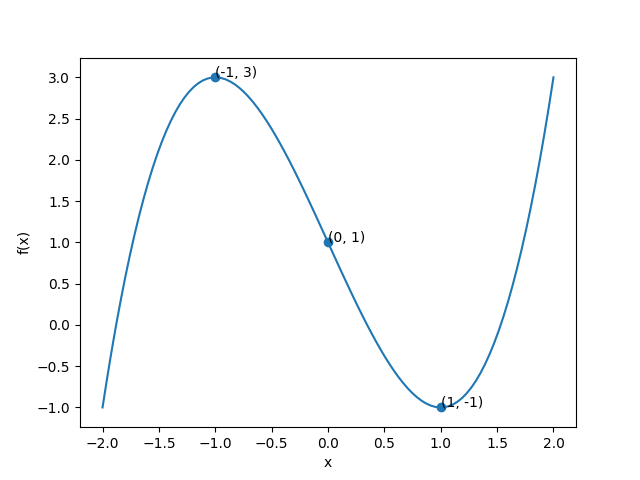
\includegraphics[scale=0.65]{595_25.png}\notag
    \end{align}
\end{problem}

\begin{problem}{27}
    $f(x) = \dfrac{8x}{x^2 + 1}$
    \begin{align}
        f'(x) &= \frac{\left(x^2 + 1\right) 8 - 8x \left(2x\right)}{\left(x^2 + 1\right)^2} \\
        &= \frac{8x^2 + 8 - 16x^2}{\left(x^2 + 1\right)^2} \\
        &= \frac{8 \left(-x^2 + 1\right)}{\left(x^2 + 1\right)^2} \\
        f''(x) &= 8 \left[\frac{\left(x^2 + 1\right)^2 \left(-2x\right) - 4x \left(-x^2 + 1\right) \left(x^2 + 1\right)}{\left(\left(x^2 + 1\right)^2\right)^2}\right] \\
        &= 8 \left[\frac{-2x^3 - 2x + 4x^3 - 4x}{\left(x^2 + 1\right)^3}\right] \\
        &= 8 \left[\frac{2x^3 - 6x}{\left(x^2 + 1\right)^3}\right] \\
        &= 16x \left[\frac{x^2 - 3}{\left(x^2 + 1\right)^3}\right] 
        \shortintertext{Critical points}
        0 &= \frac{8 \left(-x^2 + 1\right)}{\left(x^2 + 1\right)^2} \\
        0 &= -8x^2 + 8 \\
        x &= \pm\sqrt{1} \\
        f(-1) &= \frac{8 \left(-1\right)}{\left(-1\right)^2 + 1} \\
        &= \frac{-8}{2} = -4 \\
        f(1) &= \frac{8 \left(1\right)}{\left(1\right)^2 + 1} \\
        &= \frac{8}{2} = 4 
        \shortintertext{Increasing/decreasing}
        f''(-1) &= 16\left(-1\right) \left[\frac{\left(-1\right)^2 - 3}{\left(\left(-1\right)^2 + 1\right)^3}\right] \\
        &= -16 \left(\frac{-2}{8}\right) \\
        &= 4; \quad \text{Minimum @ (-1, -4)} \\
        f''(1) &= 16\left(1\right) \left[\frac{\left(1\right)^2 - 3}{\left(\left(1\right)^2 + 1\right)^3}\right] \\
        &= 16 \left(\frac{-2}{8}\right) \\
        &= -4; \quad \text{Maximum @ (1, 4)}
        \shortintertext{Inflection points}
        0 &= 16x \left[\frac{x^2 - 3}{\left(x^2 + 1\right)^3}\right] \\
        0 &= x \left(16x^2 - 48\right) \\
        x &= \pm\sqrt{3} \text{ or } 0 \\
        \shortintertext{Concavity - Test points}
        f''(-3) &= 16\left(-3\right) \left[\frac{\left(-3\right)^2 - 3}{\left(\left(-3\right)^2 + 1\right)^3}\right] = -0.288 < 0 \quad \text{concave down } (-\infty, 0) \\
        f''(0) &= 16\left(0\right) \left[\frac{\left(0\right)^2 - 3}{\left(\left(0\right)^2 + 1\right)^3}\right] = 0 \quad \text{point of inflection} \\
        f''(3) &= 16\left(3\right) \left[\frac{\left(3\right)^2 - 3}{\left(\left(3\right)^2 + 1\right)^3}\right] = 0.288 > 0 \quad \text{concave up } (0, \infty) \\
        &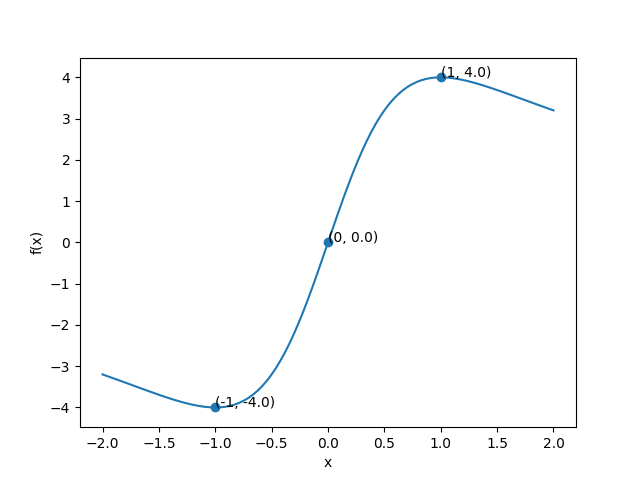
\includegraphics[scale=0.65]{595_27.png}\notag
    \end{align}
\end{problem}

\Problem{Find the absolute maximum and minimum values, if the exist, over the indicated interval.
If no interval is indicated, consider the entire real number line.}

\begin{problem}{29}
    $f(x) = 3x^2 - 6x - 4$
    \begin{align}
        f'(x) &= 6x - 6 \\
        0 &= 6x - 6 \\
        x &= 1 \\
        f(1) &= 3 - 6 - 4 = -7 \\
        f''(x) &= 6 \\
        (1, 6) &= \text{Minimum}
    \end{align}
\end{problem}

\begin{problem}{31}
    $f(x) = \frac{1}{3} x^3 - x^2 - 3x + 5; \quad [-2, 0]$
    \begin{align}
        f'(x) &= x^2 - 2x - 3; \quad [-2, 0] \\
        0 &= x^2 - 2x - 3; \quad [-2, 0] \\
        x &= \frac{2 \pm \sqrt{4 - 4\left(1\right)\left(-3\right)}}{2} \\
        &= \frac{2 \pm \sqrt{16}}{2} \\
        &= \frac{6}{2} \text{ or } \frac{-2}{2} \\
        &= 3 \text{ or } -1 \\
        f(-1) &= -\frac{1}{3} - 1 + 3 + 5 \\
        &= -\frac{5}{15} - \frac{15}{15} + \frac{45}{15} + \frac{75}{15} \\
        &= \frac{100}{15} = \frac{20}{3} \\
        f''(x) &= 2x - 2 \\
        f''(-1) &= -2 - 2 \\
        \left(-1, \frac{20}{3}\right) &= \text{Maximum}
    \end{align}
\end{problem}

\begin{problem}{32}
    \textbf{Business: maximizing profit.}
    For custom sweatshirts, Detailed Clothing's total revenue and total cost in dollars, are given by
    $$R(x) = 4x^2 + 11x + 110,$$
    $$C(x) = 4.2x^2 + 5x + 10.$$
    Find the number of sweatshirts, $x$, that must be produced and sold in order to maximize profit.
    \begin{align}
        P(x) &= R(x) - C(x) = 4x^2 + 11x + 110 - 4.2x^2 - 5x - 10 \\
        &= 0.2x^2 + 6x + 100 \\
        P'(x) &= 0.4x + 6 \\
        0 &= 0.4x + 6 \\
        x &= \frac{6}{0.4} = 15 \\
        P(15) &= 0.2\left(15\right)^2 + 6\left(15\right) + 100 = 235 \\
        P''(15) &= 0.4 \\
        (15, 235) &= \text{Minimum}
    \end{align}
\end{problem}

\end{document}

